%%%%%%%%%%%%%%%%%%%%%%%%%%%%%%%%%%%%%%%%%%%%%%%%%%%%%%%%%%%%%%%%%%%%%%%%%%%
%% This file is part of the book
%%
%% Algorithmic Graph Theory
%% http://code.google.com/p/graph-theory-algorithms-book/
%%
%% Copyright (C) 2009, 2010, 2011 Minh Van Nguyen <nguyenminh2@gmail.com>
%%
%% See the file COPYING for copying conditions.
%%%%%%%%%%%%%%%%%%%%%%%%%%%%%%%%%%%%%%%%%%%%%%%%%%%%%%%%%%%%%%%%%%%%%%%%%%%

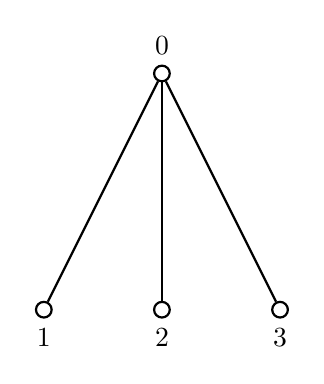
\begin{tikzpicture}
[nodedecorate/.style={shape=circle,inner sep=2pt,draw,thick},%
  linedecorate/.style={-,thick},scale=1.5]
%% nodes or vertices
\foreach \nodename/\direction/\navigate/\x/\y in {1/below/south/0/0,
  2/below/south/1/0, 3/below/south/2/0, 0/above/north/1/2}
{
  \node (\nodename) at (\x,\y) [nodedecorate] {};
  \node [\direction] at (\nodename.\navigate) {$\nodename$};
}
%% edges or lines
\path
\foreach \startnode/\endnode in {0/1, 0/2, 0/3} {
  (\startnode) edge[linedecorate] node {} (\endnode)
};
\end{tikzpicture}
